\documentclass[logos,parttoc,mainlanguage=english,morelanguage=french]{orsay-thesis}
%Text encoding and fonts
\usepackage[latin1]{inputenc}
\usepackage[T1]{fontenc}
% \usepackage{hyperref}

%########################################################################
% Title page
%########################################################################

%Thesis author
\author{Oscar Roberto \textsc{BLANCO GARC�A}}

%Title for main language (french)
\title{Beam dynamics in the final focus of the CLIC future linear collider project}
%Titles for other languages
\title[english]{Dynamique du faisceau dans las section finale de focalisation du futur collissionneur lin�aire}
% \title[german]{My German thesis title}
% \title[italian]{My Italian thesis title}

%Keywords for main language (french)
\keywords{Some keywords}
%Keywords for other languages languages
\keywords[english]{Blabla, blabla, blabla, blabla, blabla, blabla, blabla}
\keywords[german]{Blabla, blabla, blabla, blabla, blabla, blabla, blabla}
\keywords[italian]{Blabla, blabla, blabla, blabla, blabla, blabla, blabla}

%Order number of the thesis
\ordernumber{1234}

%Date of defense
\date{xx Xxxxxxxxx xxxx}

%You define the commission member list using \addcommissionmember (mandatory) with an optional role (eg: president, supervisor, etc...)
\addcommissionmember{M.}{Aaaaa}{Bbbbbbbb}
\addcommissionmember{M.}{Ccccccccc}{Dddddddddd}
\addcommissionmember[Directeur de th�se]{M.}{Eee}{Fffff}
\addcommissionmember{M.}{Ggggggggg}{Hhhhhhh}
\addcommissionmember[Pr�sident du jury]{M.}{Iiii}{Jjjjjjjjjjjj}
\addcommissionmember{M.}{Kkkkkkkkkkkk}{Llllll}

%If some referees are not part of the commission, you can add them in a separate list with \addreferee (optional)
\addreferee{M.}{Mmmmmmmm}{Nnnnnnnn}
\addreferee{M.}{Oooooooooo}{Pppppppp}

%########################################################################
% Document start
%########################################################################

\begin{document}

%Print title NOW
\maketitle%

%Disable page numbering
\pagestyle{empty}

%########################################################################
% Multilingual abstracts
%########################################################################

% %French abstract:
% \begin{abstract}
% \begin{abstract}[english]
The exploration of new physics in the TeV scale with precision measurements requires lepton colliders providing high luminosities to obtain enough statistics for the data analysis. In order to achieve design luminosity values, linear colliders feature nanometer beam spot sizes at the Interaction~Point~(IP).\par
In addition to several effects affecting the luminosity, three main issues to achieve the beam size demagnification in the Final Focus Section (FFS) of the accelerator are the chromaticity correction, the synchrotron radiation effects and the correction of the lattice errors.\par
The current linear collider projects, CLIC and ILC, have lattices designed using the local or non-local chromaticity correction schemes. A new chromaticity correction scheme, called non-interleaved, is proposed to the local and non-local chromaticity corrections for CLIC. This lattice is designed and diagnosed, where the main issue in the current state of lattice design is the non-zero second order dispersion in the Final Doublet~(FD) region where a strong sextupole is used to correct the remaining geometrical components. It could be solved by cancelling the second order dispersion and its derivative before the FD.\par
The radiation effect can be evaluated by tracking particles through the lattice or by analytical approximations during the design stage of the lattices. In order to include both, radiation and optic parameters, during the design optimization process, two particular radiation phenomena are reviewed: the Oide effect~\cite{Oide} and the radiation caused by bending magnets~\cite{Sands}.\par
The analytical result of the radiation in bending magnets in~\cite{Sands} was generalized to the case with non-zero alpha and non-zero dispersion at the IP, required during the design and luminosity optimization process. The closed solution for one dipole and one dipole with a drift is compared with the tracking code PLACET~\cite{Placet}, resulting in the improvement of the tracking code results.\par% Finally the model validity for the FFS design is analyzed concluding an agreement within $\pm10\%$ between the theoretical contribution to beam size and the tracking.\par
In the Oide effect, radiation in the final quadrupole sets a limit on the vertical beamsize. Only for CLIC 3~TeV this limit is significant, therefore two possibilities are explored to mitigate its contribution to beam size: double the length and reduce the QD0 gradient, or the integration of a pair of octupoles before and after QD0.\par
% The best result with octupoles demonstrates vertical beam size reduction of $(4.3\pm0.5)$\%, with little or negative impact on luminosity. The correction scheme is currently limited by the phase advance and $\beta_y/\beta_x$ ratio between correctors. It may be possible to improve its performance by slicing QD0.\par
Part of the requirements of the FFS for new linear accelerators, in particular ILC, are tested in The Accelerator Test Facility (ATF). The beam size reduction using the local chromaticity correction is explored by an extension of the original design, called ATF2 with two goals: ({\textbf{goal 1}}) achieve 37~nm of vertical beam size at the IP and ({\textbf{goal 2}}) the stabilization of the IP beam position at the level of few nanometres. Since 2014 beam size of 44~nm are achieved as a regular basis at charges of about~$0.1\times10^{10}$ particules per bunch.\par
A set of three cavities (IPA, IPB and IPC), two upstream and one downstream of the nominal IP, were installed and are used to measure the beam trajectory in the IP region, thus providing enough information to reconstruct the bunch position and angle at the IP. These will be used to for beam stabilization and could detect beam drift/jitter beyond the tolerable margin and undetected optics mismatch affecting the beam size measurements.\par
The specifications required of 1~nm resolution over 10~$\mu$m dynamic range at $1.0\times10^{10}$ particules per bunch with the ATF2 nominal optics have not been yet achieved. The results of the studies in the vertical plane of the cavities calibration show linearity within 5\% over two orders of magnitude of signal attenuation. The minimum resolution achieved is just below 50~nm at~$0.4\times10^{10}$ particules per bunch with a set of electronics impossing a noise limit on resolution of 10~nm per cavity. The dynamic range is 10~$\mu$m at 10~dB attenuation and $0.4\times10^{10}$ particules per bunch, indicating the need to upgrade the electronics. The integration to the ATF tuning instruments is ongoing. Nonetheless, feedback has been tested resulting in reduction of beam jitter down to 67~nm, compatible with resolution.\par
Two improvements have been done on the system since this study. First, the horizontal and vertical planes can be analyzed simultaneouly, such that data can be checked for coupling from one plane to another. Second, filters are added to the system in order to reduce the effect of the mismatch between frequencies in the electronics down-mixing process.\par
\end{abstract}
% \end{abstract}

%Horizontal rule
\noindent\hspace*{0.35\textwidth}\hrulefill\hspace*{0.35\textwidth}\\[-\bigskipamount]

%English abstract:
\begin{abstract}[english]
\begin{abstract}[english]
The exploration of new physics in the TeV scale with precision measurements requires lepton colliders providing high luminosities to obtain enough statistics for the data analysis. In order to achieve design luminosity values, linear colliders feature nanometer beam spot sizes at the Interaction~Point~(IP).\par
In addition to several effects affecting the luminosity, three main issues to achieve the beam size demagnification in the Final Focus Section (FFS) of the accelerator are the chromaticity correction, the synchrotron radiation effects and the correction of the lattice errors.\par
The current linear collider projects, CLIC and ILC, have lattices designed using the local or non-local chromaticity correction schemes. A new chromaticity correction scheme, called non-interleaved, is proposed to the local and non-local chromaticity corrections for CLIC. This lattice is designed and diagnosed, where the main issue in the current state of lattice design is the non-zero second order dispersion in the Final Doublet~(FD) region where a strong sextupole is used to correct the remaining geometrical components. It could be solved by cancelling the second order dispersion and its derivative before the FD.\par
The radiation effect can be evaluated by tracking particles through the lattice or by analytical approximations during the design stage of the lattices. In order to include both, radiation and optic parameters, during the design optimization process, two particular radiation phenomena are reviewed: the Oide effect~\cite{Oide} and the radiation caused by bending magnets~\cite{Sands}.\par
The analytical result of the radiation in bending magnets in~\cite{Sands} was generalized to the case with non-zero alpha and non-zero dispersion at the IP, required during the design and luminosity optimization process. The closed solution for one dipole and one dipole with a drift is compared with the tracking code PLACET~\cite{Placet}, resulting in the improvement of the tracking code results.\par% Finally the model validity for the FFS design is analyzed concluding an agreement within $\pm10\%$ between the theoretical contribution to beam size and the tracking.\par
In the Oide effect, radiation in the final quadrupole sets a limit on the vertical beamsize. Only for CLIC 3~TeV this limit is significant, therefore two possibilities are explored to mitigate its contribution to beam size: double the length and reduce the QD0 gradient, or the integration of a pair of octupoles before and after QD0.\par
% The best result with octupoles demonstrates vertical beam size reduction of $(4.3\pm0.5)$\%, with little or negative impact on luminosity. The correction scheme is currently limited by the phase advance and $\beta_y/\beta_x$ ratio between correctors. It may be possible to improve its performance by slicing QD0.\par
Part of the requirements of the FFS for new linear accelerators, in particular ILC, are tested in The Accelerator Test Facility (ATF). The beam size reduction using the local chromaticity correction is explored by an extension of the original design, called ATF2 with two goals: ({\textbf{goal 1}}) achieve 37~nm of vertical beam size at the IP and ({\textbf{goal 2}}) the stabilization of the IP beam position at the level of few nanometres. Since 2014 beam size of 44~nm are achieved as a regular basis at charges of about~$0.1\times10^{10}$ particules per bunch.\par
A set of three cavities (IPA, IPB and IPC), two upstream and one downstream of the nominal IP, were installed and are used to measure the beam trajectory in the IP region, thus providing enough information to reconstruct the bunch position and angle at the IP. These will be used to for beam stabilization and could detect beam drift/jitter beyond the tolerable margin and undetected optics mismatch affecting the beam size measurements.\par
The specifications required of 1~nm resolution over 10~$\mu$m dynamic range at $1.0\times10^{10}$ particules per bunch with the ATF2 nominal optics have not been yet achieved. The results of the studies in the vertical plane of the cavities calibration show linearity within 5\% over two orders of magnitude of signal attenuation. The minimum resolution achieved is just below 50~nm at~$0.4\times10^{10}$ particules per bunch with a set of electronics impossing a noise limit on resolution of 10~nm per cavity. The dynamic range is 10~$\mu$m at 10~dB attenuation and $0.4\times10^{10}$ particules per bunch, indicating the need to upgrade the electronics. The integration to the ATF tuning instruments is ongoing. Nonetheless, feedback has been tested resulting in reduction of beam jitter down to 67~nm, compatible with resolution.\par
Two improvements have been done on the system since this study. First, the horizontal and vertical planes can be analyzed simultaneouly, such that data can be checked for coupling from one plane to another. Second, filters are added to the system in order to reduce the effect of the mismatch between frequencies in the electronics down-mixing process.\par
\end{abstract}
\end{abstract}

\pagebreak

% %German abstract:
% \begin{abstract}[german]
% \dummytext
% \end{abstract}

%Horizontal rule
\noindent\hspace*{0.35\textwidth}\hrulefill\hspace*{0.35\textwidth}\\[-\bigskipamount]

% %Italian abstract:
% \begin{abstract}[italian]
% \dummytext
% \end{abstract}

%########################################################################
% Acknowledgments
%########################################################################

\pagebreak\strut\newpage

\section*{Remerciements}
%Put the text vertically centered
\vfill
This is the night of the 10th of april 2015.\par
I'm at Gen\`eve and I've been just been kicked out from La Petite Reine because the place was closing :'D, as if I care. After two beers here are my deepest acknowledgements:
From the begining...\par
My acknowledgement to Davide, the only person who has been cool every time I talk to him. My deepest acknowledgements to Alex, I wonder how the ILC course would be if I hadn't a person to talk about how people in relationships are like airplains ... some take off in very small tarmacs, like helicopters, some others need a large starting to take off.\par
My acknowledgements to Nuria who is the most constant person in my life during the last 3 years. I hope she has got something good for her life from my way of living. My acknowledgements to Julia, the russian ... waaaaw, life feels hot and nice when you speak to her. My acknowledgement to Hector, that guy is going to have his signature in the world when CLIC-like lattices were built, I want to say that we admire Carl Sagan equally... I thought it would never happen. I want to acknowledge Javier, he is the person who get me into accelerators and it is the only subject I've been looking forward to do things for during the last 10 years. I want to send an special acknowledge to Marcin, the thrill of changing every day for our own sake is what moves us, I would like to have his energy to do stuff, cheers my friend. And now, Tenar the spanish girl who appeared in the moment I most enjoyed it. Tenar, my life and heart is always happy when I hear from you. My biggest love during all these years, Claire. I don't know why, but that is probably the reason why my heart keeps beating when no one is around.\par
I want to thank Rogelio my director in CERN, the dynamics of his day to day is so dedicated to inspire people. Now, Philip, my director at LAL who is the person who stands for all what is right... I always admire how clear the world is for him. Of course, Andrea and Daniel, you are also here ! Daniel, the guy who knows everything about everything, so mind blowing. And Andrea, with whom would I talk about rare films and work at the same time... of course, only Andrea.\par
Finally, to all readers. Precisely today I wanted to be with Claire in the sunny afternoon, and this document kept me away from doing so. It is the moment to get right to the point, clear and neat. I know that Claire is fine, she always is... damn I love that girl.\par
All this is because of you, the reader.\par
N.B. Of course there has been some up and downs, but who cares. Time to flight !
\vfill

\newpage

%########################################################################
% Contents
%########################################################################

\strut\newpage

\tableofcontents

\newpage

%########################################################################
% Introduction
%########################################################################
%Enable page numbering
\pagestyle{fancy}
\section*{Introduction}
\addcontentsline{toc}{section}{Introduction}
\chapter*{Introduction}
\addcontentsline{toc}{chapter}{Introduction}
The triumph of the 20th century particle physics was the development of the Standard Model. Experiments determined the particle constituents of ordinary matter, and identified four forces binding matter and transforming it from one form to another. This success leads particle physicist to address even more fundamental questions, and explore deeper mysteries in science.\par
The Standard Model includes a third component beyond particles and forces, the Higgs mechanism. The Higgs mechanism permeates the universe, giving mass to the particles, and breaking the electro-weak force in two, the electromagnetic and the weak forces.\par
\begin{figure}[!hbt]
\centering
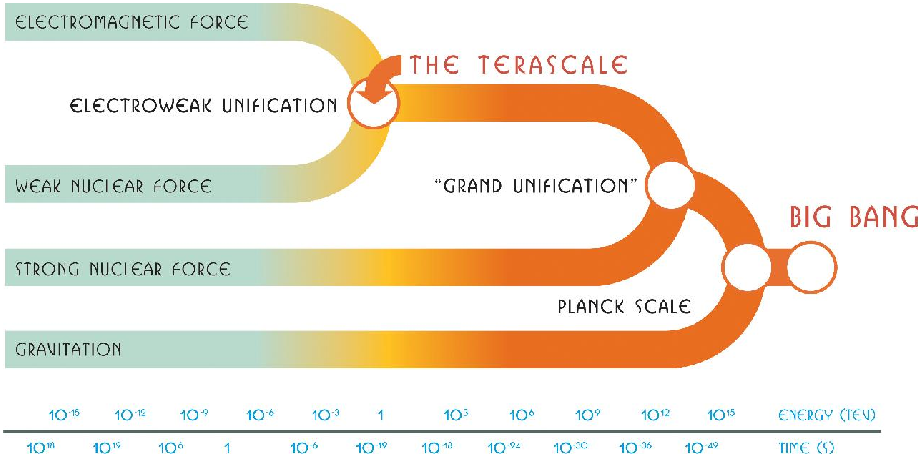
\includegraphics[scale=0.8,angle=0]{energyforce.pdf}\caption{The electromagnetic and electro-weak forces unify at the Terascale.}\label{f:energyforce}
\end{figure}
Experiments in the Terascale could test the idea that fundamental forces originate from a single unified force, see Fig. \ref{f:energyforce}, and search for evidence of a related unified origin of matter involving supersymmetry. They could distinguish among patterns of phenomena to judge different unification models, providing a telescopic view of the ultimate unification.\par
% \section*{The exploration of high energy physics}
% \addcontentsline{toc}{section}{The exploration of high energy physics}
There are two ways to explore the subatomic world, the first is to go to higher energy to discover new particles and measure their properties, the second is to increase the precision of the measurements to detect rare processes and make detailed studies.\par
The LHC allows the exploration of the electroweak symmetry breaking mechanism and other physical phenomena at the TeV scale, like the CP violation problem, the quark gluon plasma at the search of new physics beyond the Standard Model such as supersymmetry (SUSY) among others. The future linear collider beam energy will be determined by the LHC discoveries.\par
\textbf{Higgs searches:} The 4th of July of 2012, in a seminar held at CERN, the collaborations of the Experiments CMS and ATLAS presented an update of the Higgs of the Higgs searches status. At a confidence level of 4.9$\sigma$ for CMS \cite{TheCMSCollaboration21122012}, and 5.1$\sigma$ for ATLAS \cite{TheATLASCollaboration21122012} from the Higgsless Standard Model, signals of a boson with a mass around $m_h=125$~GeV were found with a strong spin-0 indication and coupling parameters consistent with the properties of the Standard Model Higgs Particle. First results on various rare production decay modes have been obtained but more data is needed to observe these models. Many analyses are ongoing and more updates are constantly presented.\par
\textbf{Heavy Flavour and CP Violation:} The experiments of the LHC, led by the LHCb, have carried out several important findings and measurements in the heavy flavour sector. New previously unobserved states have been observed for the very first time during the last years like the states $X_b$, $\Xi_a$ and $\Lambda_s^0$. Also the measurement of the quantum numbers of the states $X(3872)$ with $J^{PC}=1^{++}$, have been determined to the 8$\sigma$ level. The CP violation of the oscillation in D and B mesons have been measured to the 9.1$\sigma$ confidence level discovering the same violation in $B_s$ systems. The CP angle $\gamma$ is known with a precision without precedents ($\gamma=(67\pm12)$\textdegree). Finally, some very rare decays like $B_s\rightarrow\mu^+\mu^-$, $B^0\rightarrow K^*\mu^+\mu^-$ and $D_s^+\rightarrow\pi^+\mu^+\mu^-$ have been observed, with possible implications on the analysis of new physics.\par
\textbf{Quark-gluon Plasma:} The quark-gluon plasma is produced in ultra-relativistic heavy ion collisions. The conditions observed at the LHC experiments (ALICE, ATLAS and CMS) are in agreement with the observations carried out at RHIC. It has been confirmed that the hydrodynamics model helps in the understanding of the behaviour of the processes occurred during the collision. It is still far from being completely understood.\par
\textbf{SUSY and Dark Matter searches:} One of the problem that arises is the stabilization of the Higgs mass and its divergence when quantum divergence is considered. The solution involves a new principle of nature called supersymmetry (SUSY), a new symmetry that unifies bosons and fermions. After data collected during 2011 and 2012, SUSY searches at the LHC did not find any evidence of any light superpartner (squark or gluino) and it has pushed their mass limits beyond 1~TeV with the constrained model~\cite{Kraml:2012er}.\par
\vspace*{0.6cm}
The Second run of the LHC at 13~TeV will provide more information about the physics at high energies.\par

\section*{Circular or linear colliders}
\addcontentsline{toc}{section}{Circular or linear colliders}
Higher energies have been usually explored with hadron colliders and the precision measurements has been done afterwards by lepton colliders, however, lepton circular colliders are limited by radiation. When particles traverse magnetic fields they emmit photons and this photons make the beam loose energy per turn given by
\begin{equation}
 \Delta E_{turn}=\frac{E^4}{3\rho m_0^4c^8}
\end{equation}
where $m_0$ is the rest mass of the particle, $c$ is the speed of light, $\rho$ is the curvature radius to the trajectory produced by the magnet and $E$ is the beam energy. The highest energy lepton collision, 209~GeV, have been reached with electron and positron coliding beams in LEP at CERN.  In spite of the 27~km circumference of LEP the beam energy was limited by synchrotron radiation losses, just compensated by a powerfull superconducting RF system providing up to 3640~MV per revolution \cite{Assmann:549223}.\par
% \section{Purpose of a linear collider}

\subsection*{The requirements of high energy physics,The linear colliders (CLIC, ILC),The Accelerator Test Facility (ATF)}
\addcontentsline{toc}{subsection}{The requirements of high energy physics,The linear colliders (CLIC, ILC),The Accelerator Test Facility (ATF)}
% \subsection*{The linear colliders}
% \addcontentsline{toc}{subsection}{}
% \subsection*{The Accelerator Test Facility (ATF)}
% \addcontentsline{toc}{subsection}{The Accelerator Test Facility (ATF)}
%########################################################################
% First part
%########################################################################
\part{The beam position monitors at ATF2}
The first chapter...???
\section{The cavity BPM theory}
\subsection{Modes, transversal planes, sensitivity}
\section{IP-BPM mechanical, electrical and processing system description}
\subsection{System specifications for the ATF2 line}
\section{The installation and test}
The first section ... ???
\subsection{Installation}
\subsection{System test}
\section{Conclusions, Results and Perspectives}
The first subsection... ???
%########################################################################
% Second part
%########################################################################
\part{Final focus design for small beam size}
\section{Chromaticity correction}
\subsection{The telescopic design and the Chromaticity correction methods}
\subsection{Chromaticity minimization in the Final Doublet (FD)}
\section{Radiation in Bending Magnets}
\subsection{Theory of radiation in a bending magnet}
\subsection{Generalization for dispersive regions}
\section{Oide effect}
\subsection{Focusing limit (Oide effect)}
\subsection{Mitigation on the beam size impact}
\newpage
%########################################################################
% Conclusions
%########################################################################
\part{Conclusions}
%########################################################################
% Bibliography
%########################################################################
\thispagestyle{empty}
\strut\newpage
\addcontentsline{toc}{section}{R�f�rences}
\begin{thebibliography}{100}
\labelwidth=4em
\addtolength\leftskip{25pt}
\setlength\labelsep{0pt}
\addtolength\parskip{\smallskipamount}
\bibitem[AAA]{AAA}{Blablabla, blablablabla, blablablabla, blablablabla.}
\bibitem[BBB]{BBB}{Blablabla, blablablabla, blablablabla, blablablabla.}
\bibitem[CCC]{CCC}{Blablabla, blablablabla, blablablabla, blablablabla.}
\bibitem[DDD]{DDD}{Blablabla, blablablabla, blablablabla, blablablabla.}
\bibitem[EEE]{EEE}{Blablabla, blablablabla, blablablabla, blablablabla.}
\bibitem[FFF]{FFF}{Blablabla, blablablabla, blablablabla, blablablabla.}
\end{thebibliography}

\end{document}

%########################################################################
% Document end
%########################################################################
